
\documentclass[11pt]{article}
\usepackage{amsmath,amssymb,amsthm}
\usepackage{times,inconsolata}
\usepackage{graphicx}
\usepackage[margin=1in]{geometry}
\usepackage{fancyhdr}
\usepackage[document]{ragged2e}
\setlength{\parindent}{0pt}
\setlength{\parskip}{5pt plus 1pt}
\setlength{\headheight}{13.6pt}
\newcommand\question[2]{\vspace{.25in}\hrule\textbf{#1: #2}\vspace{.5em}\hrule\vspace{.10in}}
\renewcommand\part[1]{\vspace{.10in}\textbf{(#1)}}
\newcommand\problem{\vspace{.10in}\textbf{Problem: }}
\newcommand\algorithm{\vspace{.10in}\textbf{Algorithm: }}
\newcommand\result{\vspace{.10in}\textbf{Result: }}
\newcommand\analysis{\vspace{.10in}\textbf{Analysis: }}
\pagestyle{fancyplain}
\lhead{\textbf{Chan-Ching Hsu}}
\chead{\textbf{Data Clustering Problem}}
\rhead{\today}
\begin{document}\raggedright

\justify
\question{1}{k-means}

\problem Use k-means with k=2 and k=3 to cluster the data. When using k=2, start with data points 9 and 15 as initial seeds. When using k=2, start with data points 6, 9 and 15 as initial seeds.

\result
\begin{figure}[h]
\centering
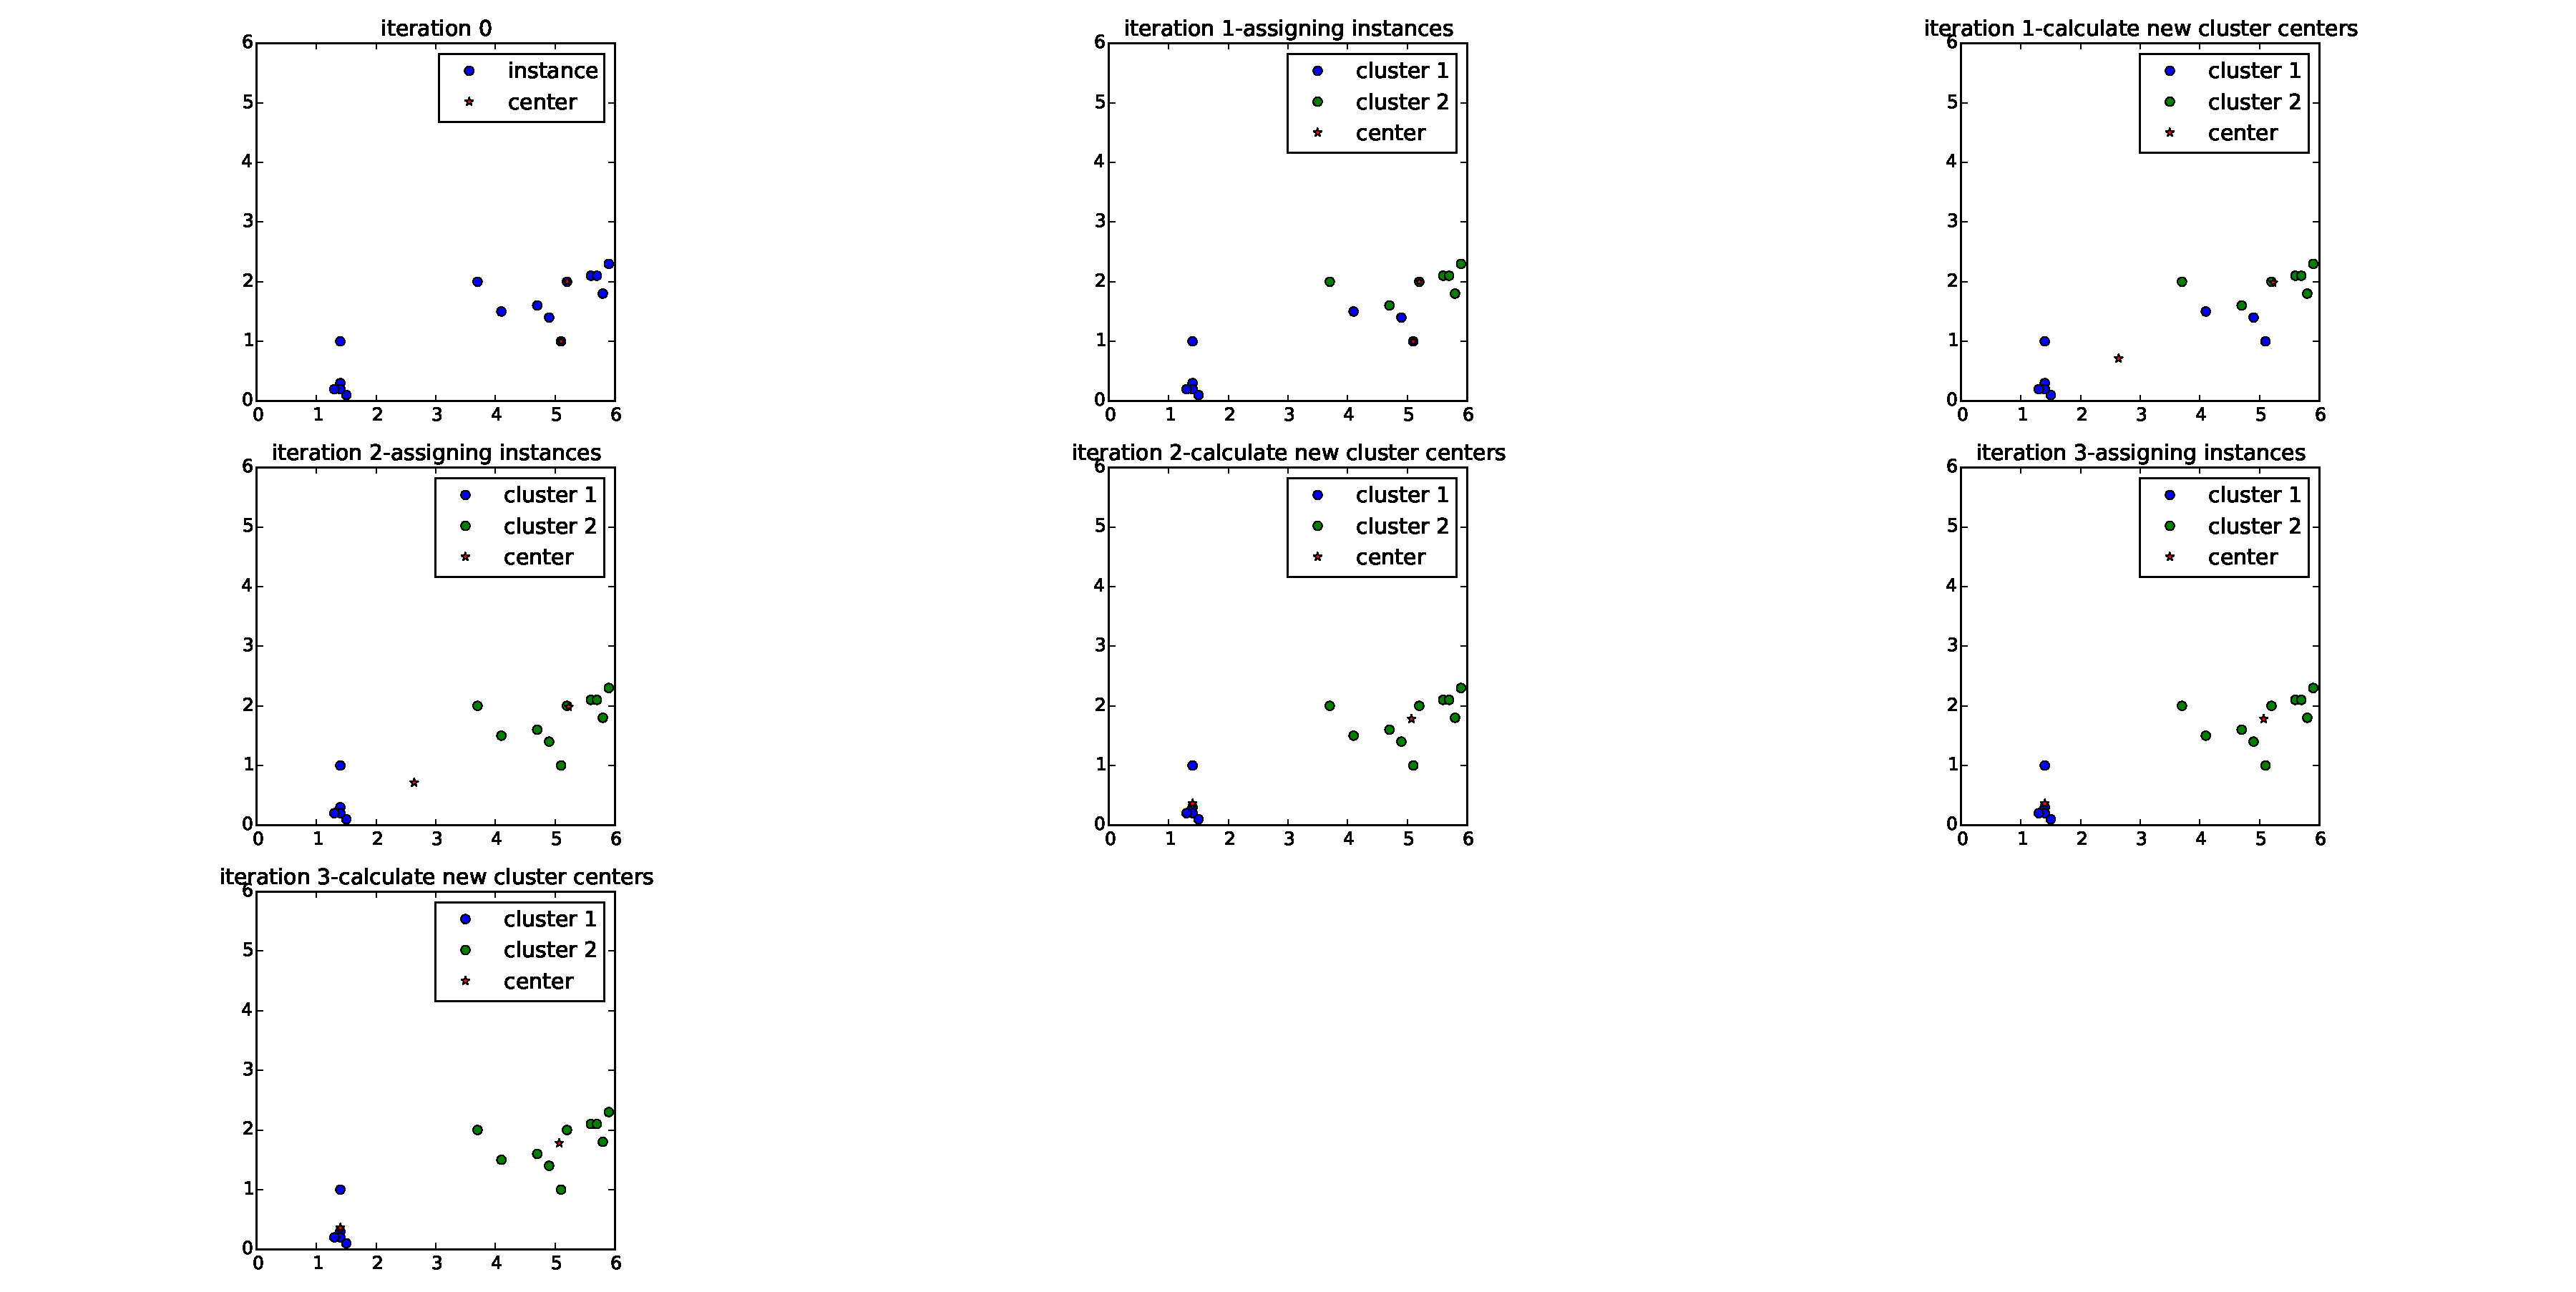
\includegraphics[width=\textwidth]{k2.pdf}
\caption{k=2, data points 9 and 15 as initial seeds}
\label{convergence1}
\end{figure}

\begin{figure}[h]
\centering
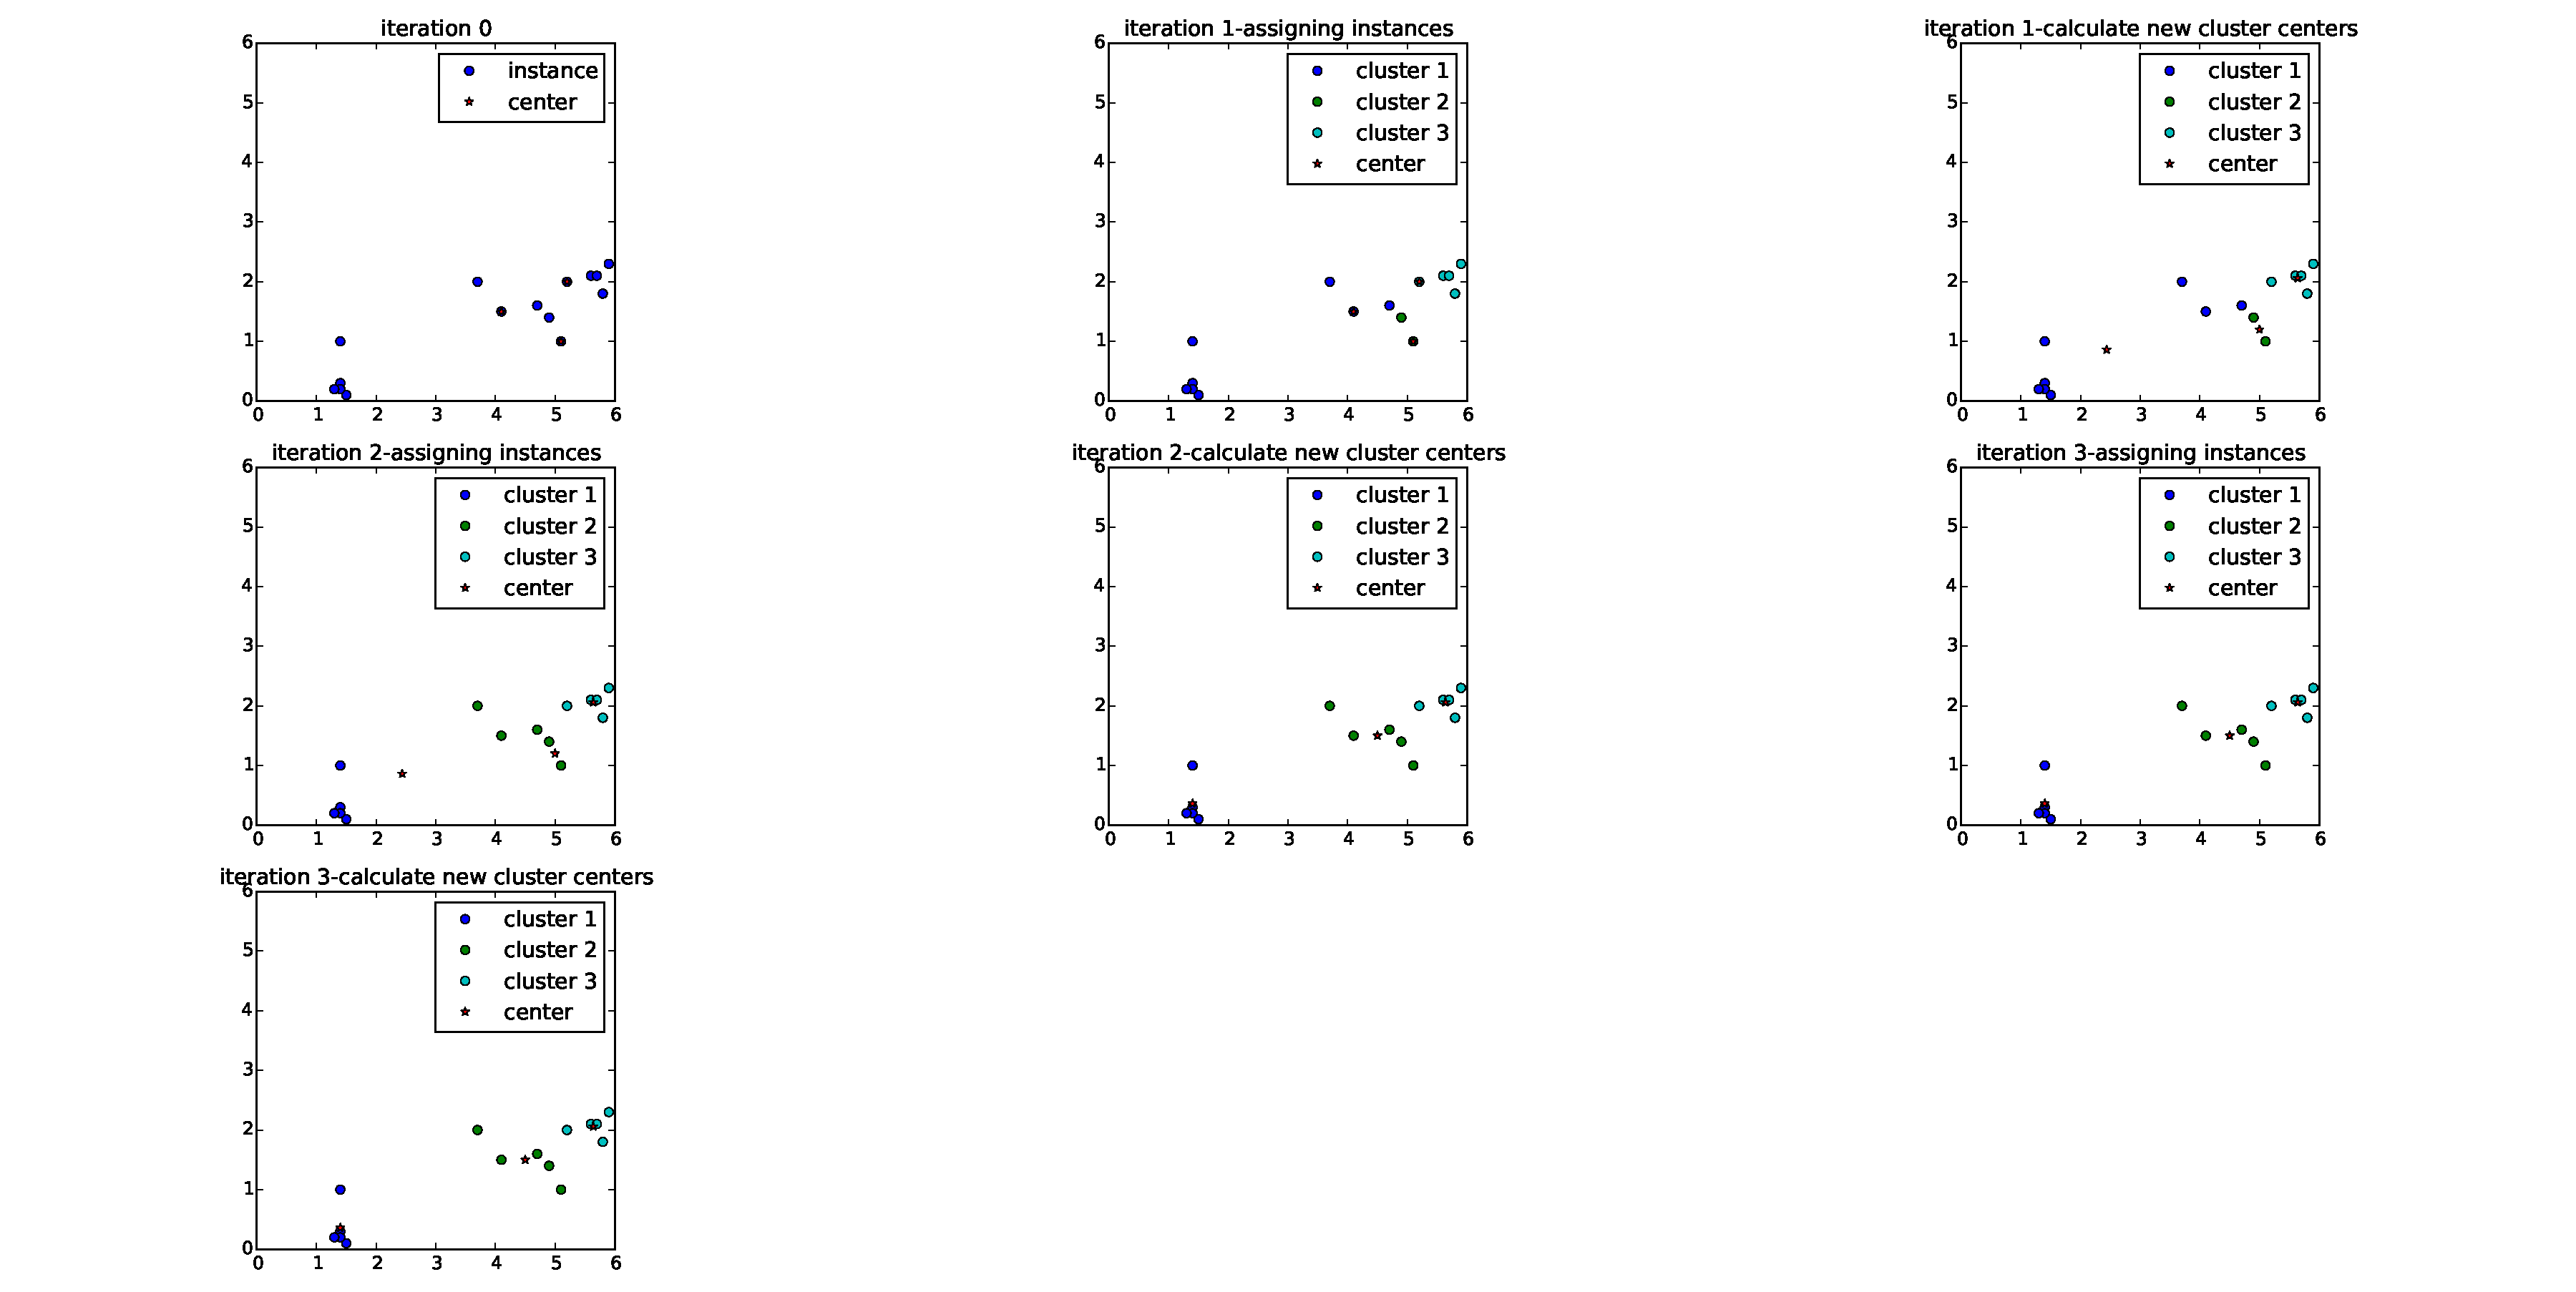
\includegraphics[width=\textwidth]{k3.pdf}
\caption{k=3, data points 6, 9 and 15 as initial seeds}
\label{convergence1}
\end{figure}
\clearpage
\question{2}{single-link agglomerative clustering}

\problem Use single-link agglomerative clustering to cluster the data. From the hierarchy, identify the clusters obtained if partitioning the data into 2 clusters and if partitioning the data into 3 clusters.

\result
\begin{figure}[h]
\centering
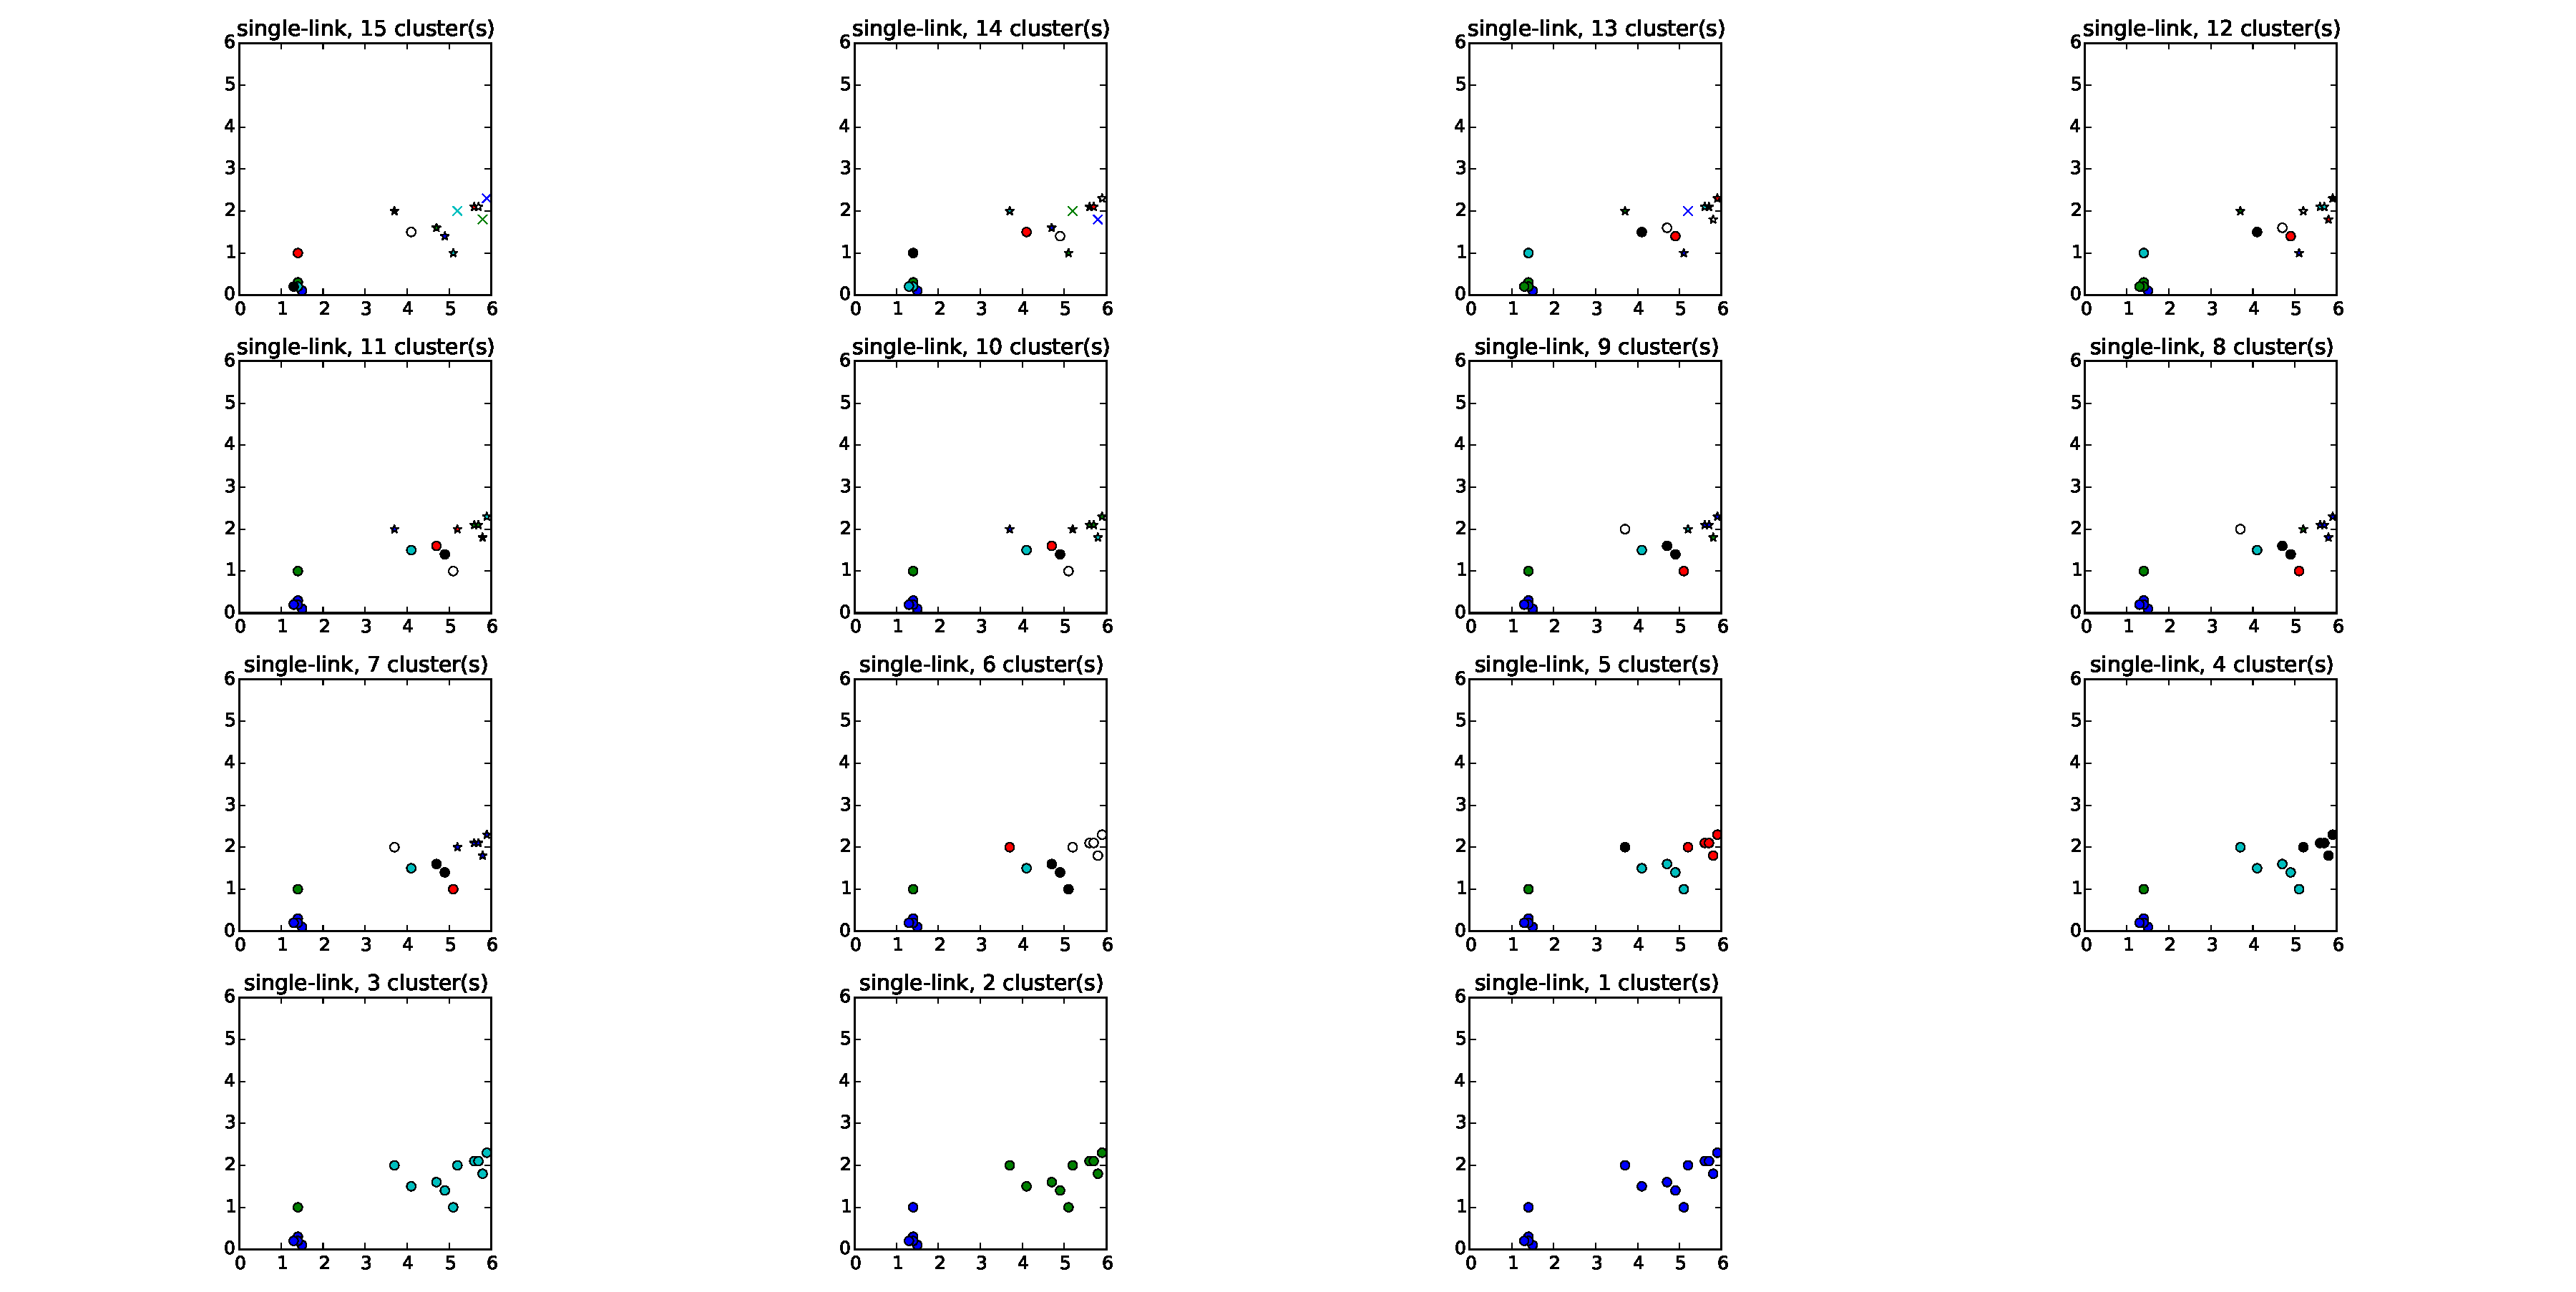
\includegraphics[width=\textwidth]{single.pdf}
\caption{Single-link Agglomerative Clustering}
\label{convergence1}
\end{figure}
\clearpage




\question{3}{complete-link agglomerative clustering}

\problem Use complete-link agglomerative clustering to cluster the data. From the hierarchy, identify the clusters obtained if partitioning the data into 2 clusters and if partitioning the data into 3 clusters.

\result
\begin{figure}[h]
\centering
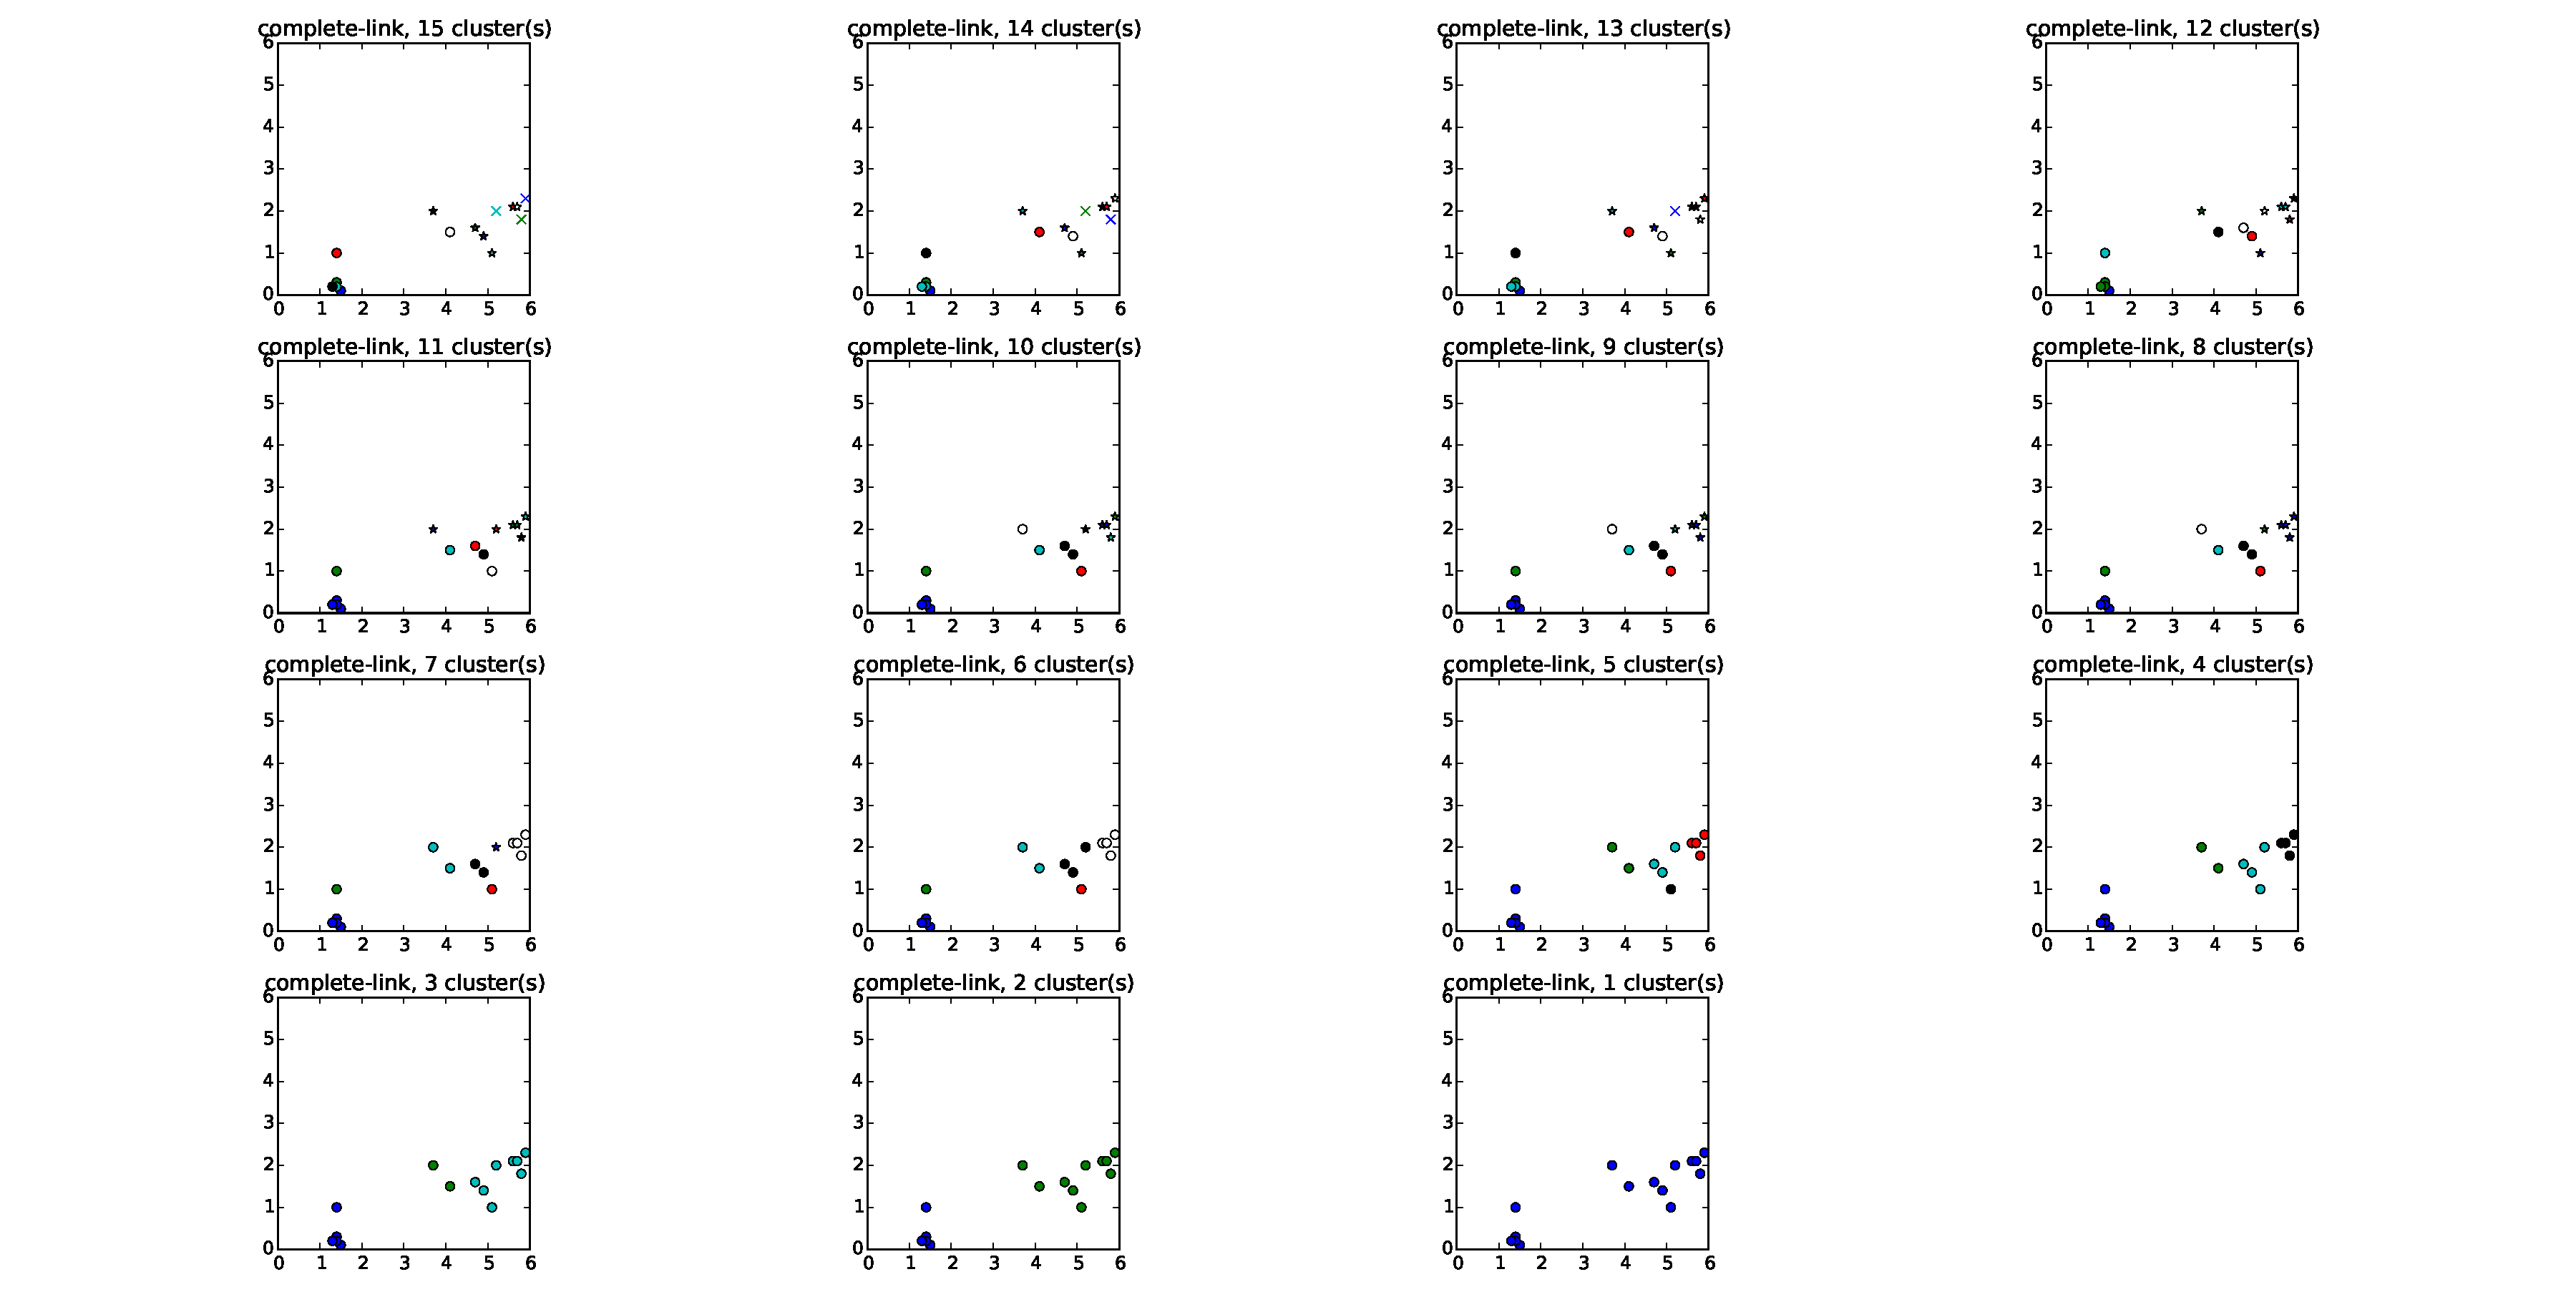
\includegraphics[width=\textwidth]{complete.pdf}
\caption{Complete-link Agglomerative Clustering}
\label{convergence1}
\end{figure}
\end{document}
